\section{Verteilte Datenverarbeitung}

Um die Belastung der Host-CPU zu reduzieren, sollen Audio-Verarbeitungsaufgaben an externe SBCs über Gigabit-Ethernet verteilt werden. Auf der Host-CPU arbeitet das Audio Plug-in als Master-Knoten. Für den Host-DAW sollte die Verteilung der Audio-Verarbeitungsaufgaben vollkommen unsichtbar sein. Der Master-Knoten empfängt MIDI- und Audiodaten vom Host-DAW und gibt die Ergebnisse zurück wie jedes andere Audio-Plug-in.

Im Gegensatz zu anderen dezentralen Verarbeitungssystemen, wo große Datenmengen an Rechenknoten in Paketen verteilt werden, bekommt das Plug-in in sehr kurzen regelmäßigen Abständen  Zugriff auf einen kleinen Pufferspeicher an Audiodaten. Das Plug-in muss in kurzer Zeit die Daten verarbeiten und zurückgeben an die Host DAW-Anwendung, bevor der nächste Puffer bereitsteht. Dies schränkt die Möglichkeiten  der Verteilung von Bearbeitungsaufträgen ein.

Es gibt verschiedene Arten, Verarbeitungsaufgaben zu parallelisieren. Jede Plug-in-Instanz könnte den gesamten Auftrag an einen Rechenknoten delegieren wie in Abbildung~\ref{fig:one_to_one} dargestellt. Besteht eine Verarbeitungsaufgabe aus mehreren, in Serie geschalteten, Verarbeitungsblöcken, dann könnte jeder Block einem Rechenknoten zugeteilt werden, wie in Abbildung\ref{fig:perproccessor} dargestellt. Speziell bei einem virtuellen Synthesizer-Plug-in könnte jede gespielte Stimme seinem eigenen Rechenknoten zugeteilt werden, siehe Abbildung~\ref{fig:perproccessor}.

\begin{figure}[H]
    \centering
    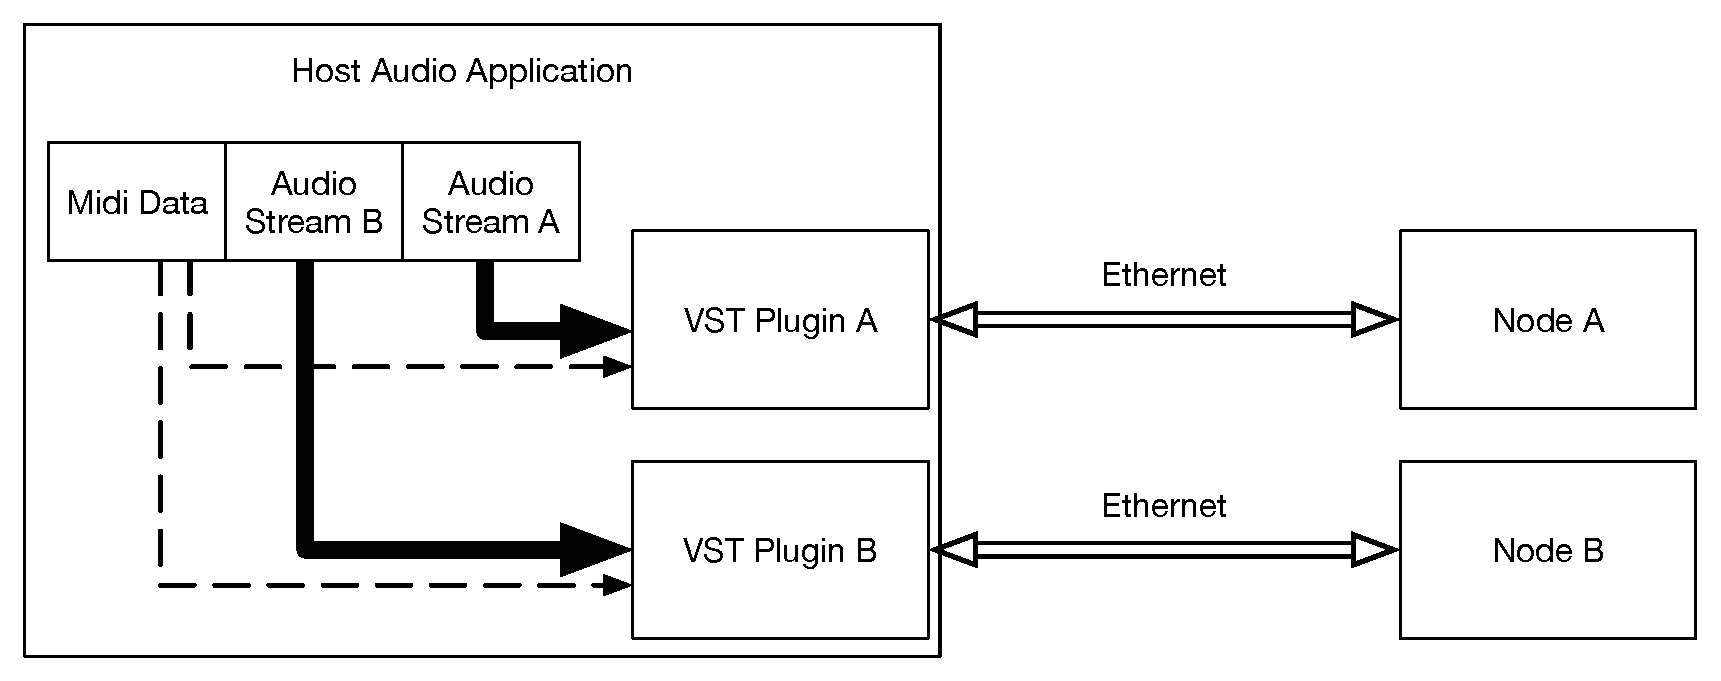
\includegraphics[width=\textwidth]{assets/distribution_1to1.pdf}
    \caption{Jedes Plug-in an einen Knoten verteilt}
    \label{fig:one_to_one}
\end{figure}

\begin{figure}[H]
    \centering
    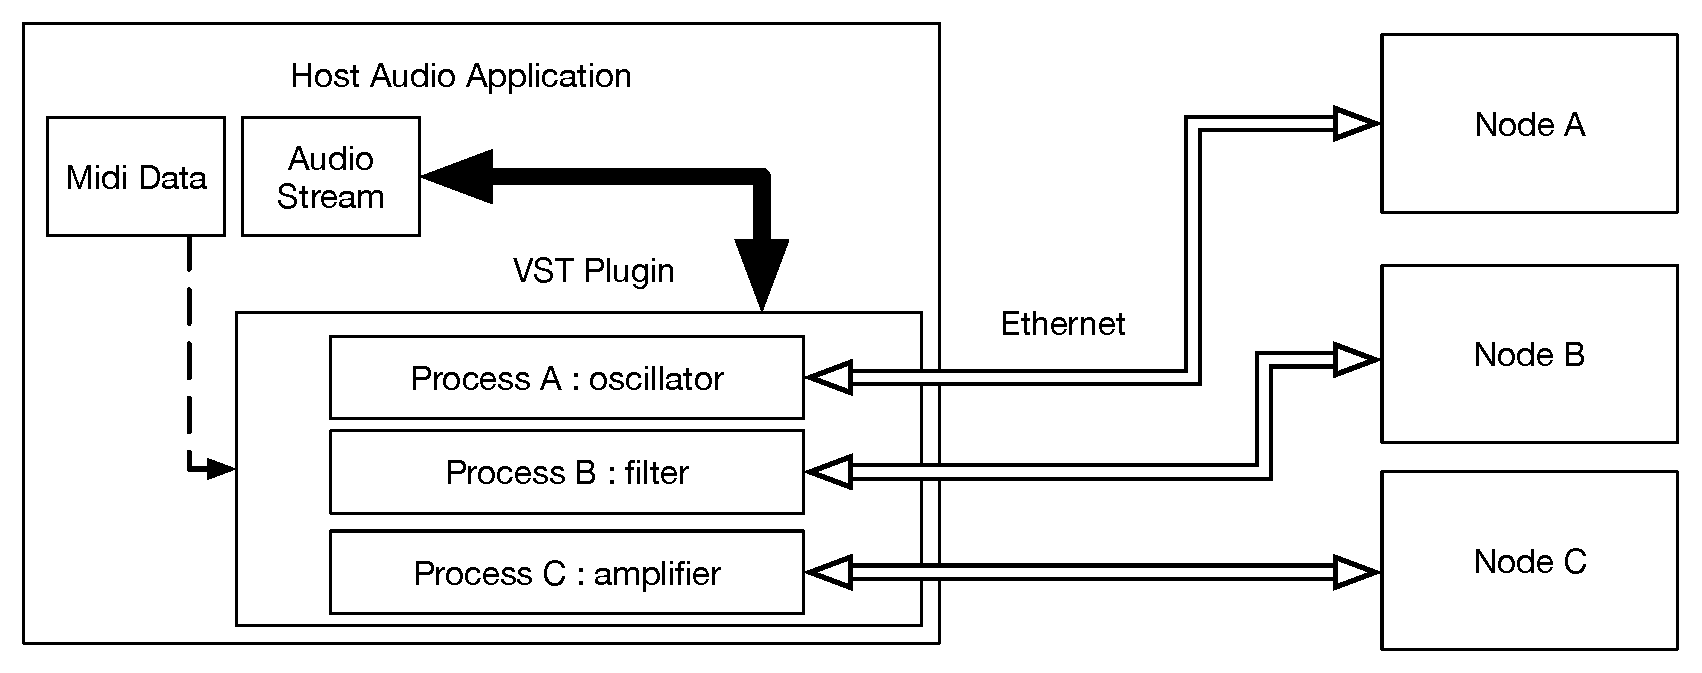
\includegraphics[width=\textwidth]{assets/distribution_perprocessor.pdf}
    \caption{Jeder Verarbeitungsblock an einen Knoten verteilt}
    \label{fig:perproccessor}
\end{figure}

\begin{figure}[H]
    \centering
    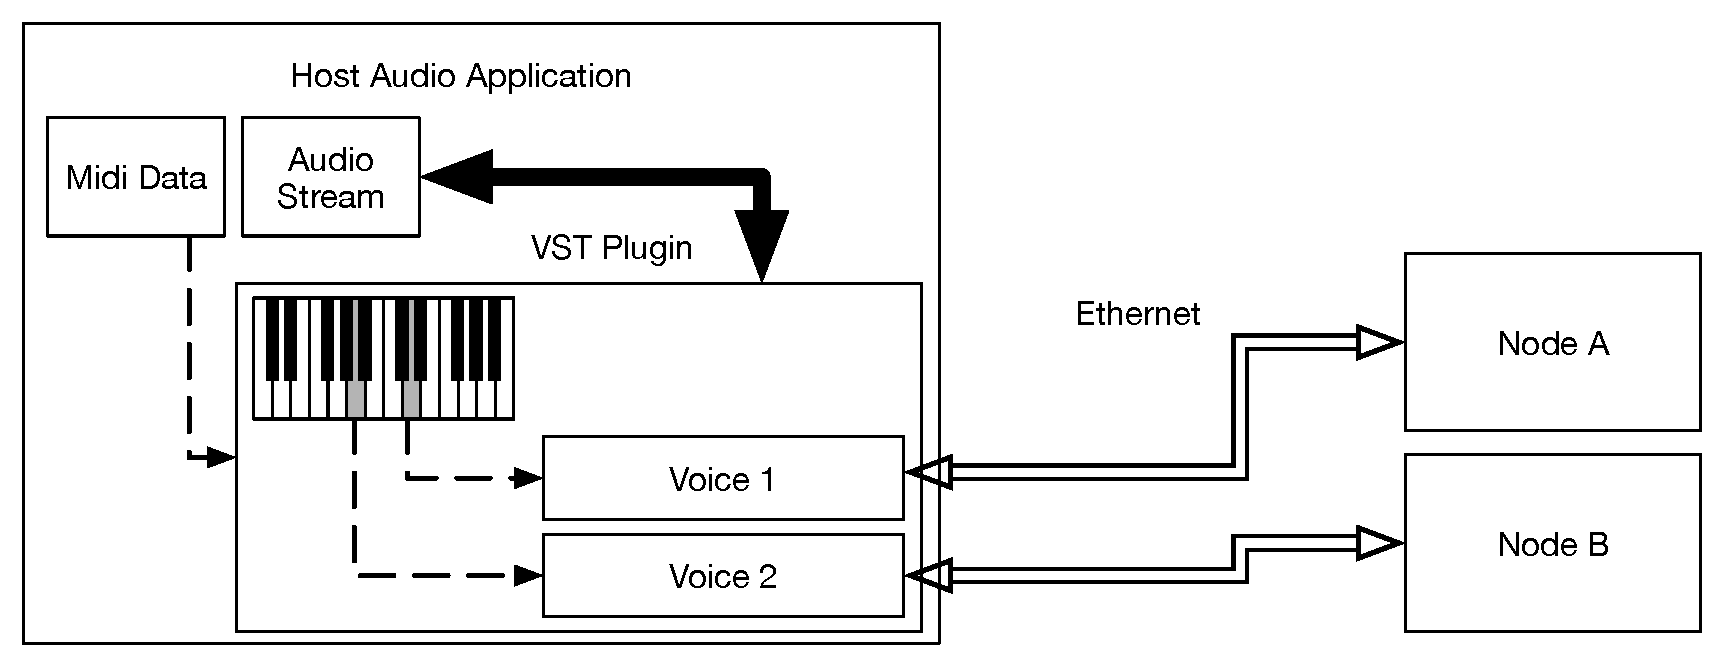
\includegraphics[width=\textwidth]{assets/distribute_byvoice.pdf}
    \caption{Jede Synth-Stimme an einen Knoten verteilt}
    \label{fig:pervoice}
\end{figure}

Für dieses Projekt wird die zweite Option implementiert aus  Gründen der Testbarkeit, auch wenn dies vielleicht nicht die effizienteste Implementierung ist.